% Emacs settings: -*-mode: latex; TeX-master: "manual.tex"; -*-

\chapter{Instrument examples}
\label{s:instrument}

In this section, we present a few example instruments, supplied with the \MCX distribution.
\begin{enumerate}
\item A model of a laboratory SAXS-instrument designed to mimic the instrument at \Lifelong built by SAXSLAB Aps.
\item An verision of the ESRF ID11 material science beamline, including models of the new transfocator devices.
\item A theoretical beamline to explore the idea of "pink" beam using CRLs.
\end{enumerate}


\subsection{SAXS at \Lifelong}
\label{ss:saxs}


\subsection{ESRF ID11}
\label{ss:id11}

\subsection{model Be-CRL beamline}
\label{ss:be-crl}


%Then, we give a longer description of three selected
%instruments. We present the \MCX\ versions of
%the Ris\o\ standard triple axis spectrometer TAS1 (\ref{s:TAS1})
%and the ISIS time-of-flight spectrometer PRISMA (\ref{s:PRISMA}).
%Before that, however, we present one example of a component
%test instrument: the instrument to test the component
%{\bfseries V\_sample} (\ref{s:V-instr}).
%%
%%The source text for the three instrument definitions
%%is listed in Appendix~\ref{instcode}.
%These instrument files are included in the \MCX\ distribution
%in the \verb+examples/+ directory.
%Most of the instrument examples there-in may be executed automatically throught the \MCX\ self-test procedure (see section~\ref{s:testing}).
%The list of instrument examples has been extended considerably, see
%the ``Neutron Site'' menu in mcgui (See page \ref{p:neutronsite}).
%\section{A quick tour of instrument examples}
%\label{s:quick-tour-instr}
%
%\subsection{Neutron site: Brookhaven}
%
%The former Brookhaven reactor hosted the H8 triple-axis spectrometer. This latter was modelled in order to cross-check the NISP, Vitess, Restrax, McStas and IDEAS neutron propagation Monte Carlo codes. Results were published in \textit{Neutron News} {\bfseries 13} (No. 4), 24-29 (2002).
%
%\subsection{Neutron site: Tools}
%
%This caterory currently contains a special \verb+Histogrammer+ that can read any event file from Vitess, MCNP, tripoli and McStas in order to produce histograms of any type. This is a very powerful tool to analyse sparse huge events data sets.
%
%\subsection{Neutron site: ILL}
%
%Cold and thermal guide models are given in the ILL neutron site. Descriptions are very accurate, based on actual drawings, including all elements with curvature and gaps. Simulated capture fluxes were found in very good agreement with measurements.
%
%Additionally, the \verb+IN12+ triple-axis instrument has been detailed, in its year 2005 configuration. It is located at the end of the H15 cold guide. sample is a Vanadium rod.
%
%The \verb+IN6+ instrument is an hybrid time-of-flight with 3 monochromators and a Fermi chopper. Sample is an isotropic scatterer (liquid). It makes use of the SPLIT keyword to enhance statistics.
%
%The \verb+ILL_TOF_Env+ example is a simple neutron pulse (e.g. from a chopper system coming out of IN5, IN4 or IN5) illuminating a sample, with a container around and a cylinder shaped sample environment.
%
%\subsection{Neutron site: tests}
%
%This large set of examples shows simple instruments using particular components (samples, polarized beams, detectors). They may be used as starting point for further more complex models.
%
%\subsection{Neutron site: ISIS}
%
%You will find here examples of ISIS instruments, some of them using the ISIS moderator component (obtained from MCNP computations).
%
%\subsection{Neutron site: Risoe}
%
%This section contains former Risoe instruments, which constitue the default test series for the \MCX\ distribution.
%
%\subsection{Neutron site: PSI}
%
%The Focus time-of-flight instrument is, with the ILL IN6 and IN12 models, the most advanced example. It as been built from drawings, including the guide and all optics elements. Simulated capture fluxes were found in good agreement with measurements.
%
%\subsection{Neutron site: Tutorial}
%
%A typical diffractometer including a powder sample and a Rescal-type triple-axis models are in this category. Instrument parameters enable models to cope with most existing instruments of these classes. The TAS model includes a basic in-plane UB-matrix transformation. It may be used to estimate the resolution functions of a TAS configuration.
%
%\subsection{Neutron site: ESS}
%
%This section contains design studies for a future, long-pulsed european spallation source. The only contents is currently the \verb+ESS_IN5_reprate+ instrument for simulating an IN5-TYPE (cold chopper) multi-frame spectrometer for the long-pulsed ESS. (Also serves as example instrument for \verb+Tunneling_sample.comp+.)
%
%\section{A test instrument for the component V\_sample}
%\label{s:V-instr}
%This is one of many test instruments written with the
%purpose of testing the individual components. We have picked
%this instrument both to present an
%example test instrument and because it despite its simplicity
%has produced quite non-trivial results.
%
%The instrument consists of a narrow source,
%a 60' collimator, a V-sample shaped as a hollow cylinder
%with height 15 mm, inner diameter 16 mm, and outer diameter 24 mm
%at a distance of 1 m from the source.
%The sample is in turn surrounded by an unphysical $4\pi$-PSD
%monitor with $50 \times 100$ pixels and a radius of $10^{6}$ m.
%The set-up is shown in figure~\ref{f:V-instr}.
%
%\begin{figure}
%  \begin{center}
%    \psfrag{Source}{Source}
%    \psfrag{Collimator}{Collimator}
%    \psfrag{Vanadium}{Vanadium}
%    \psfrag{4pipsd}{$4\pi$ PSD}
%    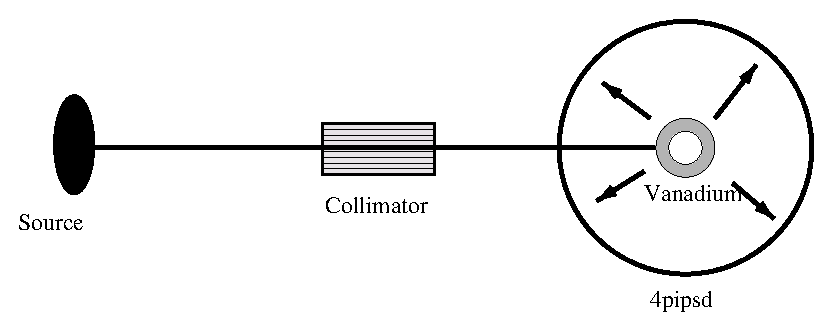
\includegraphics[width=0.9\textwidth]{figures/vanadium.eps}
%  \end{center}
%\caption{A sketch of the test instrument for the component
%V\_sample.}
%\label{f:V-instr}
%\end{figure}
%
%\subsection{Scattering from the V-sample test instrument}
%\label{s:vanadium-result}
%
%In figure \ref{f:V-results}, we present the radial distribution
%of the scatting from an evenly illuminated V-sample,
%as seen by a spherical PSD.
%It is interesting to note that the variation in the
%scattering intensity is as large as 10\%. This is an effect
%of anisotropic attenuation of the beam in the cylindrical sample.
%
%\begin{figure}
%  \begin{center}
%    \includegraphics[width=0.6\textwidth]{figures/vanadium-surf-2.eps}
%  \end{center}
%\caption{Scattering from a V-sample, measured by a spherical
%  PSD. The sphere has been transformed onto a plane and the intensity is
%  plotted as the third dimension. }
%\label{f:V-results}
%\end{figure}
%
%
%
%\section{The triple axis spectrometer TAS1}
%\label{s:TAS1}
%With this instrument definition, we have tried to create
%a very detailed model of the conventional cold-source
%triple-axis spectrometer TAS1 at the now closed neutron source DR3 of
%Ris\o\ National Laboratory.
%Except for the cold source itself, all components
%used have quite realistic properties. Furthermore, the overall
%geometry of the instrument has been adapted from
%the detailed technical drawings of the real spectrometer.
%The TAS 1 simulation was the first detailed work
%performed with the \MCX\ package.
%For further details see reference~\cite{tas1_report}.
%
%At the spectrometer, the channel from the cold source
%to the monochromator is asymmetric, since the first
%part of the channel is shared with other instruments.
%In the instrument definition, this is represented by
%three slits.
%For the cold source, we use a flat energy
%distribution (component {\bfseries Source\_flat})
%focusing on the third slit.
%
%The real monochromator consist of seven blades, vertically focusing on
%the sample. The angle of curvature is constant so that the focusing is
%perfect at 5.0 meV (20.0 meV for 2nd order reflections) for a 1$\times$1~cm$^2$
%sample. This is modeled directly in the instrument definition using
%seven {\bfseries Monochromator} components. The mosaicity of the pyrolytic
%graphite crystals is nominally 30' (FWHM) in both directions.  However, the
%simulations indicated that the horisontal mosaicities of both
%monochromator and analyser were more likely 45'. This was used for all
%mosaicities in the final instrument definition.
%
%The monochromator scattering angle, in effect determining the incoming
%neutron energy, is for the real spectrometer fixed by four holes in the
%shielding, corresponding to the energies 3.6, 5.0, 7.2, and 13.7~meV for
%first order neutrons.  In the instrument definition, we have adapted the
%angle corresponding to 5.0~meV in order to test the simulations against
%measurements performed on the spectrometer.
%
%The width of the exit channel from the monochromator may
%be narrowed down from initially 40~mm
%to 20~mm by an insert piece. In the simulations, we have chosen
%the 20~mm option and modeled the channel with two slits to match
%the experimental set-up.
%
%In the test experiments, we used two standard samples:
%An Al$_2$O$_3$ powder sample and a vanadium sample. The instrument
%definitions use either of these samples of the correct
%size. Both samples are chosen to focus on the opening aperture of
%collimator 2 (the one between the sample and the analyser).
%Two slits, one before and one after the sample,
%are in the instrument definition set to the opening values which
%were used in the experiments.
%
%The analyser of the spectrometer is flat and made from
%pyrolytic graphite. It is placed between an entry and
%an exit channel, the latter leading to a single detector.
%All this has been copied into the instrument definition.
%
%On the spectrometer, Soller collimators may be inserted
%at three positions: Between monochromator and sample,
%between sample and analyser, and between analyser and detector.
%In our instrument definition, we have used 30', 28', and 67' collimators
%on these three positions, respectively.
%
%An illustration of the TAS1 instrument
%is shown in figure~\ref{f:TAS1}.
%Test results and data from the real spectrometer are shown
%in Appendix~\ref{data:TAS1}.
%
%\begin{figure}
%  \begin{center}
%    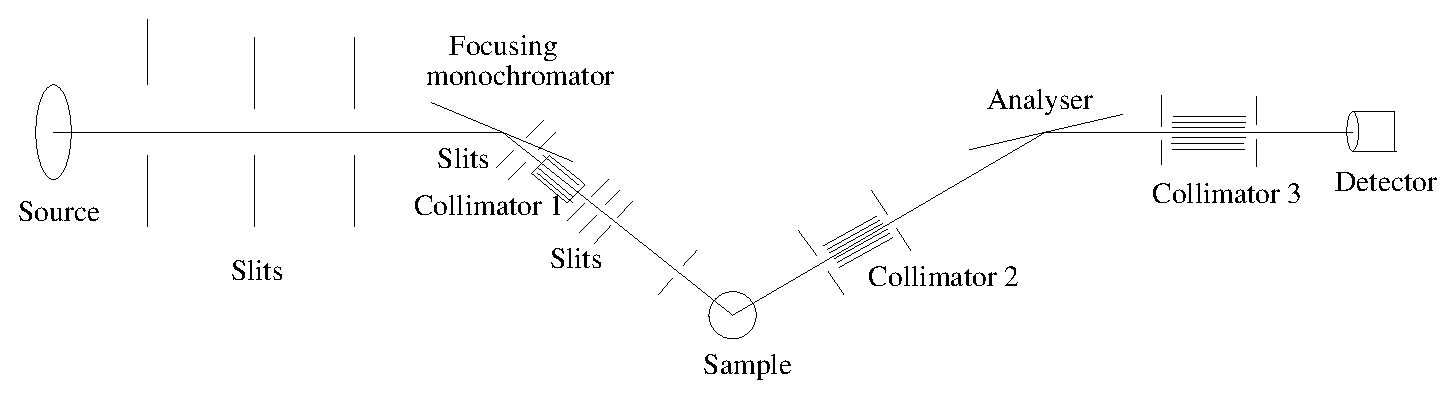
\includegraphics[width=0.9\textwidth]{figures/tas1.eps}
%  \end{center}
%\caption{A sketch of the TAS1 instrument.}
%\label{f:TAS1}
%\end{figure}
%
%\subsection{Simulated and measured resolution of TAS1}
%\label{data:TAS1}
%
%In order to test the \MCX\ package on a qualitative level,
%we have performed a very detailed comparison of a simulation with a
%standard experiment from TAS1. The measurement series
%constitutes a complete alignment of the spectrometer,
%using the direct beam and scattering from V and Al$_2$O$_3$
%samples at an incoming energy of 20.0~meV, using the second order
%scattering from the monochromator.
%
%In these simulations, we have tried to reproduce
%every alignment scan with respect to position and width
%of the peaks, whereas we have not tried to compare
%absolute intensities. Below, we show a few comparisons
%of the simulations and the measurements.
%
%Figure \ref{f:2t_direct} shows a scan of
%$2\theta_m$ on the collimated direct beam in two-axis mode.
%A \hbox{1 mm} slit is placed on the sample position.
%Both the measured width and non-Gaussian peak shape
%are well reproduced by the \MCX\ simulations.
%
%\begin{figure}
%  \begin{center}
%    \includegraphics[width=0.6\textwidth]{figures/tas1-2T.eps}
%  \end{center}
%\caption{TAS1: Scans of $2\theta_s$ in the direct beam with 1 mm slit on the
%  sample position.
%"$\times$": measurements, "o": simulations, scaled to the same intensity
%Collimations: open-30'-open-open.}
%\label{f:2t_direct}
%\end{figure}
%
%In contrast, a simulated $2\theta_a$ scan in triple-axis
%mode on a V-sample showed a surprising offset from 0 degrees.
%However, a simulation with a PSD
%on the sample position showed that the beam center was 1.5~mm
%off from the center of the sample, and this was important
%since the beam was no wider than the sample itself.
%A subsequent centering of the beam resulted in a nice
%agreement between simulation and measurements.
%For a comparison on a slightly different instrument
%(analyser-detector collimator inserted),
%see Figure~\ref{f:v_2ta_zero}.
%
%%\begin{figure}
%%  \begin{center}
%%    \includegraphics[width=0.6\textwidth]{figures/vanadium-plot-1.eps}
%%  \end{center}
%%\caption{First simulated $2\theta_a$ scan on a vanadium sample.
%%Collimations: open-30'-28'-open.}
%%\label{f:v_2ta_offset}
%%\end{figure}
%
%\begin{figure}
%  \begin{center}
%    \includegraphics[width=0.6\textwidth]{figures/vanadium-plot-2.eps}
%  \end{center}
%\caption{TAS1: Corrected $2\theta_a$ scan on a V-sample.
%Collimations: open-30'-28'-67'.
%"$\times$": measurements, "o": simulations.}
%\label{f:v_2ta_zero}
%\end{figure}
%
%The result of a $2\theta_s$ scan on an Al$_2$O$_3$
%powder sample in two-axis mode is shown in Figure \ref{f:al2o3}.
%Both for the scan in focusing mode (+ $-$ +)
%and for the one in defocusing mode (+ + +) (not shown),
%the agreement between simulation and experiment is excellent.
%
%\begin{figure}
%  \begin{center}
%    \includegraphics[width=0.6\textwidth]{figures/al2o3-focus.eps}
%  \end{center}
%\caption{TAS1: $2\theta_s$ scans on Al$_2$O$_3$ in two-axis, focusing mode.
%Collimations: open-30'-28'-67'.
%"$\times$": measurements, "o": simulations.
%A constant background is added to the simulated data.}
%\label{f:al2o3}
%\end{figure}
%
%As a final result, we present a scan of the energy
%transfer $E_a = \hbar \omega$ on a V-sample.
%The data are shown in Figure \ref{f:v_ea}.
%
%\begin{figure}
%  \begin{center}
%    \includegraphics[width=0.6\textwidth]{figures/ea-scan.eps}
%  \end{center}
%\caption{TAS1: Scans of the analyser energy on a V-sample.
%Collimations: open-30'-28'-67'.
%"$\times$": measurements, "o": simulations.}
%\label{f:v_ea}
%\end{figure}
%
%
%\section{The time-of-flight spectrometer PRISMA}
%\label{s:PRISMA}
%
%In order to test the time-of-flight aspect of \MCX, we have
%in collaboration with Mark Hagen, now at SNS, written a simple
%simulation of a time-of-flight instrument loosely based on the ISIS
%spectrometer PRISMA. The simulation was used to investigate the effect
%of using a RITA-style analyser instead of the normal PRISMA backend.
%
%We have used the simple time-of-flight source {\bfseries Tof\_source}.
%The neutrons pass through a
%beam channel and scatter off from a vanadium sample, pass through
%a collimator on to the analyser.
%The RITA-style analyser consists of seven analyser crystals
%that can be rotated independently around a vertical axis. After the
%analysers we have placed a PSD and a time-of-flight detector.
%
%To illustrate some of the things that can be done in a simulation as
%opposed to a real-life experiment, this example instrument further
%discriminates between
%the scattering off each individual analyser crystal
%when the neutron hits the detector. The
%analyser component is modified so that a global variable
%\verb+neu_color+ registers which
%crystal scatters the neutron ray. The detector component
%is then modified to construct seven different time-of-flight histograms,
%one for each crystal (see the source code for the instrument
%for details). One way to think of this is that
%the analyser blades paint a color on each neutron which is then
%observed in the detector.
%An illustration of the instrument is shown in figure~\ref{f:PRISMA}.
%Test results are shown in Appendix~\ref{data:PRISMA}.
%
%\begin{figure}[h]
%  \begin{center}
%    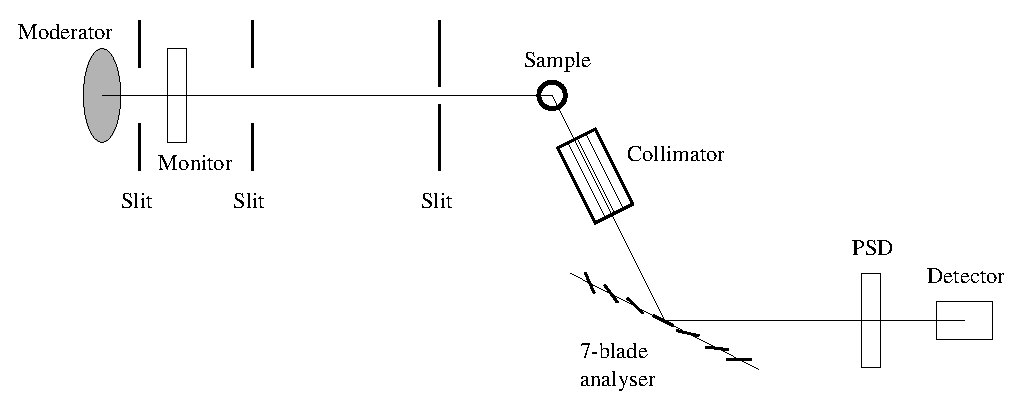
\includegraphics[width=0.9\textwidth]{figures/prisma2.eps}
%  \end{center}
%\caption{A sketch of the PRISMA instrument.}
%\label{f:PRISMA}
%\end{figure}
%
%\subsection{Simple spectra from the PRISMA instrument}
%\label{data:PRISMA}
%
%A plot from the detector in the PRISMA simulation is shown in Figure
%\ref{f:PRISMAdata}. These results were obtained with each analyser blade
%rotated one degree relative to the previous one. The separation of the
%spectra of the different analyser blades is caused by different energy
%of scattered neutrons and different flight path length from source to
%detector.  We have not performed any quantitative analysis of the data.
%
%\begin{figure}
%  \begin{center}
%    \includegraphics[width=0.6\textwidth]{figures/prisma2-a.eps}
%  \end{center}
%\caption{Test result from PRISMA instrument using ``colored
%  neutrons''. Each graph shows the neutrons scattered from one analyser blade.}
%\label{f:PRISMAdata}
%\end{figure}
